\chapter{CSW graph-theoretic approach to quantum correlations}
\lhead{\emph{CSW graph-theoretic approach to quantum correlations}}
\label{sec:csw}

In \cite{Cabello2014}, the authors propose a graph-theoretic approach to classifying the statistics of an arbitrary correlation experiment that aims to determine the value of some linear combination of probabilities. In particular, \cite{Cabello2014} identifies a hierarchical structure that classifies correlations as classical (KS non-contextual), quantum, or more generally obeying the exclusivity principle \footnote{The exclusivity applies to pairwise exclusive events and bars their added probabilities from exceeding 1. We will come back to it shortly.}. This hierarchical structure is established by associating with a correlation experiment its corresponding ``exclusivity graph". The exclusivity structure obeyed by the experiment imposes non-trivial constraints on the set of permissible correlations compatible with KS non-contextuality, QM, or the exclusivity principle. In particular, upper bounds of the relevant linear combination of probabilities, within these three classes of theories, can be related to graph invariants of the experiment's exclusivity graph.

\section{Generic correlation experiments in the CSW framework}
\label{sec:correxp}
The CSW framework takes an operationalist approach to correlation experiments, in the sense that any such experiment is described in terms of a sequence of (reproducible) experimental procedures. For example, one such experimental procedure may be to prepare the system in a certain way. If they provide the experimenter with an output (apart from the transformed system), such experimental procedures can be considered \emph{tests}. For a preparation $P$, and test $M$ with outcomes $\{k_i\}_i$, an operational theory specifies the probabilities $p(k_i\vert M,P)$. 

There may be multiple equivalent ways of preparing a system, in the sense that we can never tell the preparation procedures apart by experiment, as they yield identical probability distributions for all tests. The equivalence class of operationally indistinguishable preparation procedures $P$ defines a state. In the same manner, the equivalence class of operationally indistinguishable tests $M$ defines an observable\footnote{This identification of operationally equivalent tests and preparations parallels the operational equivalence classes we will introduce in Section \ref{sec:spekkcont}, when introducing the notion of  Spekkens contextuality.}.

We now define what it means for two observables to be compatible, or jointly measurable. While in QM two projective measurements are compatible if and only if the corresponding Hermitian operators commute, we want to define compatibility in operational terms, in order for the definition to be applicable to arbitrary operational theories.

\begin{definition}
\label{def:compat}
Two observables $M_{1}$, $M_{2}$ with outcome sets $\{k_i\}_i$ and $\{k'_i\}_{i}$, respectively, are \emph{jointly measurable} if there exists an observable $M_{12}$ with outcome set $\{k_i,k'_j\}_{i,j}$ such that:
\begin{enumerate}
\item $\forall$ preparations $P$, $\forall$ outcomes $k\in\{k_i\}_i$:\hfill\break $p(k\vert M_1,P)=\sum_{k'}p(k,k'\vert M_{12},P)$
\item $\forall$ preparations $P$, $\forall$ outcomes $k'\in\{k'_j\}_j$:\hfill\break $p(k'\vert M_2,P)=\sum_{k}p(k,k'\vert M_{12},P)$
\end{enumerate}
\end{definition}

\noindent One may think of $M_{12}$ as measuring both $M_{1}$ and $M_{2}$ simultaneously, placing the outcome of $M_{1}$ into its first and the outcome of $M_{2}$ into its second output register. By discarding one of the outcomes, we reduce $M_{12}$ to the corresponding single-outcome measurement. At the level of probability distributions, discarding one of the outcomes corresponds to a summation over all possible outcomes held by the discarded register. For QM as operational theory and projective measurements, this definition is equivalent to operator commutativity. For general quantum measurements, Definition \ref{def:compat} implies that the POVM $M_1$ and $M_2$ are obtained by coarse graining the POVM $M_{12}$ that jointly realizes both.

An \emph{event} is characterized by a list of compatible tests $(M_1, M_2, \dots, M_n)$ that yield some outcomes $(X_1, X_2, \dots, X_n)$. Let $X_1,X_2,\dots, X_n\thinspace\vert\thinspace M_1,M_2,\dots, M_n$ denote such event. Some events may be operationally equivalent, in the sense that they have the identical probability of occuring, for all initial preparations of the system. Analogous to our treatment of preparations and tests, operationally equivalent test-outcome tuples define the same event. Within QM, a state would be defined by a density operator, whereas equivalent events correspond to the same positive semi-definite operator or projector.

A correlation experiment, like the KCBS or CHSH experiment, consists of one or multiple experimenters performing subsets of compatible tests on an intial preparation $P$ of the system. For instance, in the KCBS experiment, an experimenter chooses between five measurement contexts $(i,i\oplus 1)$. We assume that an experimenter can freely choose between measurement contexts, i.e.\ subsets of compatible tests, meaning that this choice is not correlated with say the system being measured. By recording which of all could-be events occurs for many repetitions of this procedure, the experimenter(s) can determine the value of some relevant linear combination $\sum_i w_i p(\epsilon_i\vert P)$, where $w_i>0$, and $\epsilon_i$ denotes a possible event i.e.\ a set of compatible tests that yield some outcomes. Sometimes we will omit the initial preparation $P$ in our formulas. Let us now discuss what conditions and assumptions allow us to impose non-trivial constraints on correlations.

We define two events to be exclusive if they specify different outcomes for identical tests.
\begin{definition}[\cite{Amaral2018}]
\label{def:exclevents}
For outcome-repeatable tests, two events
\begin{equation*}
X_1,X_2,\dots, X_n\thinspace\vert\thinspace M_1,M_2,\dots, M_n\;\text{ and }\; X'_1,X'_2,\dots, X'_m\thinspace\vert\thinspace M'_1,M'_2,\dots, M'_m  
\end{equation*} are \emph{exclusive} if for some $i$ and $j$
\begin{equation*}
    M_i = M'_j \text{ and } X_i \neq X'_j.
\end{equation*}
\end{definition}

An important assumption that underlies the CSW framework is that all measurements are assumed to be outcome-repeatable, meaning that performing two identical tests in a consecutive manner always yields identical outcomes. As such, we can, by performing a subsequent measurement $M_i$, perfectly distinguish between two exclusive events. The assumption of outcome repeatability compells us to restrict quantum measurements to PVM, as this is not a general feature of unsharp quantum measurements. Dropping the assumption of outcome repeatability and thereby accounting for general POVM quantum measurements will not provide us with any non-trivial constraints distinguishing the set of quantum correlations from the the set of general probabilistic assignments, at least not within the CSW framework. The reason for this that the exclusivity principle, which we invoke in Section \ref{sec:cswhierarch} to obtain constraints on correlations, is in general not true for theories within which pairwise compatibility does not imply joint compatibility (Specker's ``fundamental theorem'', see Section \ref{sec:threeboxes}). There exist POVM that are pairwise compatible, but fail to satisfy joint compatibility \cite{Heunen2014}. Section \ref{sec:cswunsharp} will discuss in more detail how the CSW framework falls apart when allowing for general unsharp measurements.

For a correlation experiment with two exclusive could-be measurements events $\epsilon_1$ and $\epsilon_2$, the sum of their probabilities cannot exceed 1, for all initial preparations $P$: Take $M$ to be the test that perfectly distinguishes between $\epsilon_1$ and $\epsilon_2$, like in Definition \ref{def:exclevents}, with $\epsilon_1$ specifying the outcome $X_1$ and $\epsilon_2$ the outcome $X_2$. Imagine performing the test $M$ after one input-output round of the correlation experiment: 
\begin{align*}
1 & \geq p(\{X_1,X_2\}\vert M) \\
& \geq p(\{X_1,X_2\}\vert M, \epsilon_1)\thinspace p(\epsilon_1) + p(\{X_1,X_2\}\vert M, \epsilon_2)\thinspace p(\epsilon_2)\\
& = p(\epsilon_1)+p(\epsilon_2).
\end{align*}
The exclusivity principle extends this property to sets of pairwise exclusive events:

\begin{principle}[Exclusivity principle]\hfill\break
For a set of pairwise exclusive measurement events of a correlation experiment $\{\epsilon_i\}_i$
\begin{equation*}
    \sum_i p(\epsilon_i)\leq 1,
\end{equation*}
for all initial preparations.
\end{principle}

We denote the set of correlations that are compatible with the exclusivity principle by $E_1$.

Not all valid assignments of probabilities to events of a correlation experiment, i.e.\ probabilistic models of a correlation experiment, are compatible with the exclusivity principle. For example, consider Specker's three boxes, as introduced in Section \ref{sec:threeboxes}. The relevant linear combination of probabilities that this correlation experiment tests is
\begin{equation*}
S = \frac{1}{3}\sum_{i=1}^3\thinspace p(0,1 \thinspace\vert\thinspace i,i\oplus 1) +  \frac{1}{3}\sum_{i=1}^3\thinspace p(1,0\thinspace\vert\thinspace i\oplus 1,i).
\end{equation*}
For both sums, the events that appear are pairwise exclusive. Therefore, within theories obeying the exclusivity principle, $S$ is upper-bounded by $\frac{2}{3}$. However, by assigning the probability $\frac{1}{2}$ to each event appearing in $S$ we obtain a probability assignment that is compatible with pairwise exclusivity, but incompatible with the exclusivity principle. Furthermore, this assignment of probabilities is consistent with perfectly anti-correlated outcomes for all measurement contexts, as was considered in Section \ref{sec:threeboxes}.
While the exclusivity principle must not be true for arbitrary theories, it does apply to QM, if all measurements are projective, and by extension to KS non-contextual correlations. This can be seen by noting that exclusive events must be assigned orthogonal projectors and noting that for a set of orthogonal projectors $\{\Pi_i\}_i$, $(\thinspace\mathbb{1}-\sum_i \Pi_i\thinspace)$ is a positive semi-definite operator.
Therefore, in Section \ref{sec:cswhierarch}, we may use the exclusivity principle to impose constraints on the set of quantum (and KS non-contextual) correlations.

If we extend quantum measurements to general POVM, the exclusivity principle must no longer hold, as we just demonstrated for correlation experiments like Specker's three boxes (assign the positive operator $\frac{\mathbb{1}}{2}$ to all measurement events).

\section{The exclusivity graph of a correlation experiment}
The exclusivity graph of a correlation experiment is a convenient representation of the exclusivity structure obeyed by events that imposes constraints on what correlations are permissible within different classes of theories. 
The exclusivity graph of a correlation experiment $S=\sum_i w_i p(\epsilon_i)$ has a vertex for each measurement event $\epsilon_i$ appearing in $S$.  Furthermore, exclusive measurement events are represented as adjancent vertices, as shown in Figure \ref{fig:kcbsexclusivity} for the KCBS correlation experiment, or in Figure \ref{fig:3boxesexcl} for Specker's three boxes.


\begin{figure}
\centering
\begin{subfigure}{\textwidth}
    \centering
    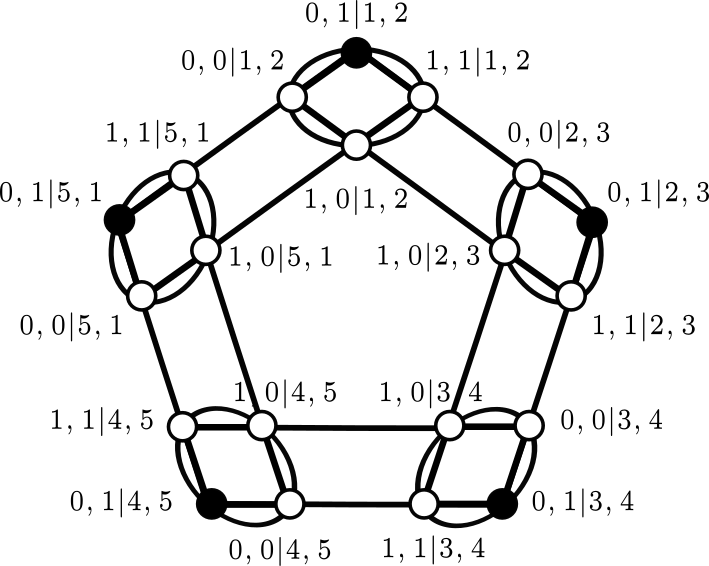
\includegraphics[width=0.6\textwidth]{images/kcbsexclusivity1.png}
    \caption{Graph depicting all events of the KCBS correlation experiment and the underlying exclusivity structure. An event is defined in terms of a measurement context and outcome tuple, and is represented by a vertex of the graph. Adjacent vertices correspond to ``mutually exclusive" events. Figure copied from \cite{Cabello2014}.}
\end{subfigure}
\break\vspace{5ex}
\begin{subfigure}{\textwidth}
    \centering 
    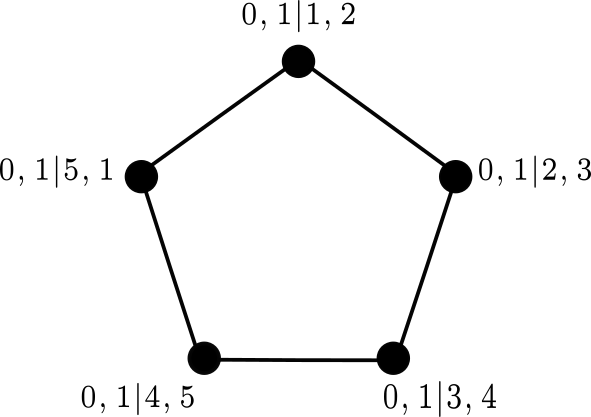
\includegraphics[width=0.6\textwidth]{images/kcbsexclusivity2.png}
    \caption{Simplified exclusivity graph for the KCBS correlation experiment. Contains only those vertices in (a) whose probabilities appear in the KCBS KS non-contextuality inequality. Figure copied from \cite{Cabello2014}.}
\end{subfigure}

\caption{KCBS exclusivity graph}
\label{fig:kcbsexclusivity}
\end{figure}


\begin{figure}
    \centering
    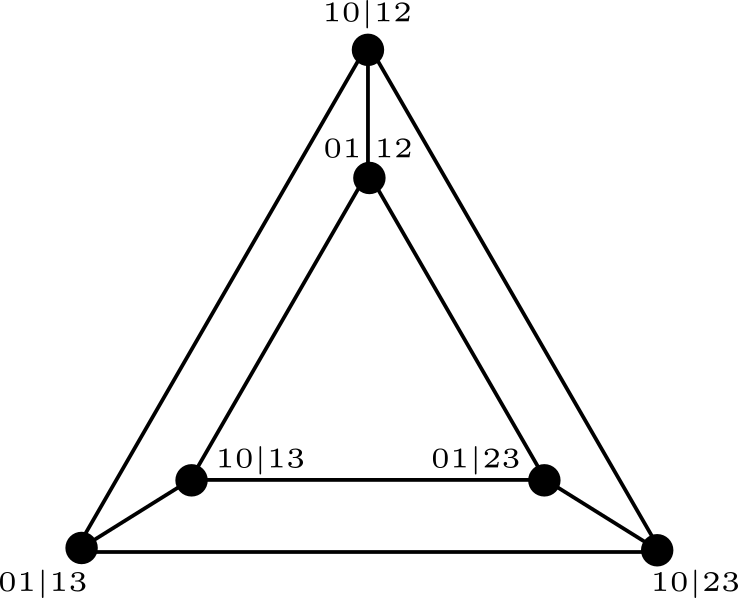
\includegraphics[width=0.5\textwidth]{images/3boxesecl.png}
    \caption{Exclusivity graph for Specker's three boxes correlations experiment, see Section \ref{sec:threeboxes}. The outcome 0 corresponds to the opened box being empty, whereas the outcome 1 corresponds to the opened box containing a gem.}
    \label{fig:3boxesexcl}
\end{figure}

\section{Hierarchical structure of correlations}
\label{sec:cswhierarch}
We will now relate upper bounds for the quantity $S$, for correlations that are compatible with KS non-contextuality, QM, or the exclusivity principle, to graph invariants of the experiment's exclusivity graph. All three graph invariants can be computed by solving a corresponding mathematical optimization problems. The proofs we present are adapted from \cite{Cabello2014}:

\begin{itemize}
    \item \textbf{KS non-contextual correlations:}
    The CSW approach decouples KS non-contextuality from the operational theory that is QM and extends it to arbitrary operational theories. For a given exclusivity graph, classical i.e.\ KS non-contextual correlations are those that can be written as a convex combination of deterministic assignments $\nu: V\mapsto\{0,1\}$ that obey the exclusivity principle, where $V$ is the vertex set of the correlation experiment. Let us verify that this extension to arbitrary operational theories is compatible with KS non-contextuality as defined in Definition \ref{def:kscontherm}: Assuming QM and projective measurements, each event defines a (distinct) projector, as we identify operationally equivalent events. Furthermore, pairwise exclusive events correspond to pairwise orthogonal projectors and can be regarded as part of the same resolution of the identity. The correlation experiment is consistent with a KS non-contextual description according to Definition \ref{def:kscontherm} if and only if all correlations are compatible with an assignment $\nu$ like above, up to convex combination. Therefore, for the case of QM as operational theory and perfectly sharp measurements, the generalized notion of classicality in \cite{Cabello2014} reduces to KS non-contextuality like in Definition \ref{def:kscontherm}.
    
    As will be discussed in Section \ref{sec:odum}, lifting the notion of KS non-contextuality as relevant criterion for non-classicality to arbitrary operational theories, and assigning outcomes in a deterministic fashion to potentially unsharp measurements, gives rise to a number of inconsistencies. Therefore, this ``incremental" \cite{Pusey2019} approach towards an operational notion of non-contextuality seems to be flawed. An alternative will be presented in Section \ref{sec:spekkensopappr}.
    
    We now wish to determine the maximal value of $S$ that is compatible with a classical description like above. For a set of pairwise adjacent vertices, the sum of the probabilities assigned to these cannot exceed 1. Only two independent vertices, meaning two vertices that are non-adjacent can both receive the valuation 1. It follows that the maximal value of $S$ is \begin{equation}
    S_{nc}=\max\limits_{U}\;\sum_{i\in U} w_i,
    \end{equation}
    where the expression is maximized over all independent sets of the exclusivity graph. This is the independence number of the (weighted) exclusivity graph. Section \ref{sec:kcbs} presents concrete values for the odd $n$-cycle scenarios, see Equation \ref{eqn:oddncycleclass}.
    
    \item \textbf{Quantum correlations:}
    The set of quantum correlations, restricting to projective measurements, is of the form\footnote{We can w.l.o.g.\ assume a pure quantum state. For mixed states $\ket{\rho_A}$, consider the purification $\Psi_{AE}$ and projectors $(\thinspace\Pi_i\otimes\mathbb{1}_E\thinspace)$.} \begin{equation*}
    p(\epsilon_i)=\expval{\Pi_i}{\Psi},
    \end{equation*}
    for some quantum state $\ket{\Psi}$ and $\Pi_{i}$ the projector corresponding to the event $\epsilon_i$. Adjacent events must be represented by orthogonal projectors:
    \begin{equation*}
        \Pi_{i}\Pi_{j} = 0 \text{ for } \epsilon_i, \epsilon_j \text{ adjancent}.
    \end{equation*}
    For an arbitrary quantum realization $\vert \Psi\rangle$, $\{\Pi_{i}\}_i$, define the vectors
    \[\ket{u_0} \coloneqq \ket{\Psi}\text{ and }\ket{u_i} \coloneqq \frac{\Pi_{i} \ket{u_0}}{\sqrt{\expval{\Pi_i}{u_0}}} \]
    
        
    The $(n+1)\times(n+1)$ Gram matrix\footnote{The Gram matrix $X$ of a set of vectors $v_1,\dots, v_n$ in an inner product space $(V,\langle \cdot, \cdot\rangle)$ is the $n\times n$ matrix with entries $X_{ij}=\bra{ v_i}\ket{ v_j}$. The Gram matrix of a set of vectors is positive semi-definite and all positive semi-definite matrices are the Gram matrix for some non-unique list of vectors. For a $n\times n$ positive semi-definite matrix $X$, we can always find a suitable list of vectors in $(\mathbb{C}^n, \langle \cdot, \cdot\rangle_{\text{std}})$, where $\langle \cdot, \cdot\rangle_{\text{std}}$ is the standard inner product, by computing the Cholesky decomposition of $X$. Acting with an arbitrary isometry $V:\mathbb{C}^n\rightarrow\mathbb{C}^d$, $d\geq n$, yields a Gram decomposition in $(\mathbb{C}^d,\langle \cdot, \cdot\rangle_{\text{std}})$.} $X$ of the vectors $\{\bra{u_i}\ket{u_0} \ket{u_i}\}_{i=0}^n$ obeys the following constraints:
    \begin{align*}
        X_{00} &= 1\,,\\
        X_{0i} &= X_{ii}\,,\\
        \text{and } X_{ij} &= 0 \text{ for $\epsilon_i$, $\epsilon_j$ adjacent} \\  
    \end{align*}
    Additionally, $\sum_i w_i X_{ii} = \sum_i w_i \abs{\expval{\Pi_i}{\Psi}}^2$, the value of the linear combination $S$ for the quantum model $\ket{\Psi}$, $\{\Pi_i\}_i$. As we can construct a Gram matrix that satisfies these constraints and which is related to $S$ like above for all quantum experiments , the maximum value of $S$, for a given exclusivity graph, that is compatible with QM is upper-bounded by the so-called Lovász semi-definite program (SDP) \cite{Bharti2019}
    \begin{alignat}{2}
    \label{eqn:lovaszsdp}
    \operatorname{max}\sum_{i=1}^n\; & w_i X_{ii} \nonumber\\
    \text{subject to } X_{ii} &=X_{01}\;,\hspace{1ex} && 1\leq i\leq n \\
    X_{ij} & = 0 \;, && \text{for } \epsilon_i,\; \epsilon_j \text{ adjacent} \nonumber\\
    X_{00} & = 1 \;,\; && X\in\mathcal{S}_{+}^{\thinspace n+1},\nonumber
    \end{alignat}
    where $\mathcal{S}_{+}^{1+n}$ is the set of positive semi-definite $(n+1)\times(n+1)$ matrices.
    
    One might naively think that the Lovász bound is tight: For an optimal solution of the Lovàsz SDP \ref{eqn:lovaszsdp}, $X^*$, with Gram decompostion $\{\ket{u_i}\}_{i=0}^n$, $S=\sum_{i=1}^n w_i X^*_{ii}$ can be realized by the quantum experiment which consists of an experimenter performing the rank-one projective measurements $\ket{\Tilde{u_i}} \bra{\Tilde{u_i}}$ on the state $\ket{\Tilde{u_0}}$, where the vectors $\{\ket{\Tilde{u}_i}\}_{i=0}^n$ are obtained by normalization:
    \begin{align*}
    p(\epsilon_i) =\operatorname{tr}(\ket{\Tilde{u}_i}\bra{\Tilde{u}_i} \ket{\Tilde{u}_0}\bra{\Tilde{u}_0}) = \abs{ \bra{\Tilde{u}_0} \ket{\Tilde{u}_i}} ^2 = \frac{\abs{ \bra{u_0} \ket{u_i}} ^2}{\bra{u_0}\ket{u_0}\bra{u_i}\ket{u_i}} = \abs{\bra{u_i}\ket{u_i}}=X_{ii},
    \end{align*}
    where $\epsilon_i\equiv 1 \thinspace\vert\thinspace \ket{\Tilde{u}_i}\bra{\Tilde{u}_i}$ and the last equality follows from the constraints a feasible solution of the Lovász SDP \ref{eqn:lovaszsdp} must satisfy.
    However, the Lovász bound on quantum correlations arising from projective measurements is in general not tight. For Bell scenarios with multiple space-like separated subsystems, the concrete physical setting of the correlation experiment imposes additional constraints on what projectors $\{\Pi_i\}_i$ are physical. In particular these have to respect locality $\Pi_i = \Pi_A^{(i)}\otimes\Pi_B^{(i)}$.
    For contextuality scenarios the Lovász bound is generally tight, as is the case for the class of odd $n$-cycle scenarios presented in Section \ref{sec:kcbs}.
    
    \item \textbf{Correlations in $E_1$:}
    The fractional packing number of the weighted exclusivity graph is defined as 
    \begin{equation*}
    \max\limits_{\{p_i\}_i}\thinspace \sum_{i\in V}w_i\thinspace p_i,    
    \end{equation*}
    where the expression is maximized over all $\{p_i\}_i$ with $p_i\geq0$ and $\sum_{i\in C} p_i\leq 1$, for all subsets $C$ of pairwise exclusive events (cliques) of the exclusivity graph. This is just the the maximum value of $S$ for correlations in $E_1$. For the KCBS inequality $E_1$ correlations can achieve 
    $\sum_{i=1}^5 p(0,1\vert i, i+1) = \frac{5}{2}.$

    
\end{itemize}

\section{What about unsharp measurements?}
\label{sec:cswunsharp}
The CSW framework falls apart when we allow for outcome unsharp measurements. In particular, as we will see in the next section, the Lovász number \ref{eqn:lovaszsdp} no longer bounds general quantum behaviours, and even trivial POVM $\{a\mathbb{1}\}_{a}$ can realize the most general probabilistic models \cite{Kunjwal2019}. In particular, they can produce violations of KS non-contextuality inequalities that exceed those achieved by just projective measurements. One arrives at the pathological conclusion that, within the CSW framework, if we do not restrict the set of measurements, all correlations are quantum (compatible with QM), yet all correlations can be produced by trivial POVM, which are intuitively classical\footnote{A trivial POVM generates a random output, totally independent of the measured system's state. One can therefore implement an operationally equivalent measurment by discarding the system and flipping some potentially biased coins.}. Thus, the hierarchical structure of correlations established in Section \ref{sec:cswhierarch} breaks down for this case. Futhermore, extending our classicality criterion, namely KS non-contextuality, to unsharp measurements is conceptually problematic and raises numerous inconsistencies, as will be discussed in Section \ref{sec:odum}.

\section{Complications that arise without space-like separation}
\label{sec:complicationscont}
Let us now comprehend in what sense trivial POVM are able to realize arbitrary probabilistic models, in particular violate KS non-contextuality inequalities, and how come one doesn't encounter the same complications for Bell-type scenarios. 

To work with a concrete example, consider the KCBS correlation experiment with exclusivity graph Figure \ref{fig:kcbsexclusivity}. We present an argument that parallels the one presented in \cite{Kunjwal2019}.
Let $(i,i\oplus1)$ denote two compatible dichotomic measurements an experimenter can perform, which we will assume to be compatible POVM. Importantly, there generally exist many joint POVM $\{M_{00}^{i,i\oplus1},M_{01}^{i,i\oplus1}, M_{10}^{i,i\oplus1},M_{11}^{i,i\oplus1}\}$, satisfying Definition \ref{def:compat}, and we cannot rule out any of these without making additional assumptions. For Bell-type correlation experiments, we can impose additional constraints due to locality, namely that compatible measurements act on local Hilbert spaces, and in particular that compatible POVM are commuting. In contrast to projective measurements, commutativity is sufficient but not necessary for two POVM to be compatible: If and only if all elements from both POVM commute, their joint POVM is uniquely determined as
\begin{equation*}
    M_{ab}=M_{a}^i M_{b}^{i\oplus1},
\end{equation*}
where $i\equiv\{M_{a}^i\}_a$ and $i\oplus1\equiv\{M_{b}^{i\oplus1}\}_b$ \cite{Kunjwal2019}.

Let us compare the possible correlations that may arise from commuting POVM to those that can arise from non-commuting, compatible POVM:

\begin{itemize}
    \item \textbf{commuting POVM (Bell-type scenarios):}
    Due to commutativity, the probability of an event $x,y\thinspace\vert\thinspace i,i\oplus 1$ can be calculated like
    \begin{equation*}
        p(x,y\thinspace\vert\thinspace i,i\oplus 1) = \operatorname{tr}(\rho\thinspace M_x^i\thinspace M_y^{i\oplus 1}).
    \end{equation*}
    For Bell tests with remote measurement contexts, the joint measurement is given by a tensor product.
    
    If we consider all POVM $i$ to be trivial, $i\equiv\{a^i_0\thinspace\mathbb{1}\thinspace,\thinspace a^i_1\thinspace\mathbb{1}\}$, then we find a joint probability distribution for all measurements $i$ that is compatible with all measureable marginal correlations for the five measurement contexts,
    \begin{equation*}
        p(x,y,z,v,w)=a^1_{x}\;a^2_{y}\;a^3_{z}\;a^4_{v}\;a^5_{w}\;,
    \end{equation*}
    where $x,\dots,w$ denote the outcomes of the five measurements $i$. Finding such a global probability distribution implies that all correlations produced by the experiment are KS non-contextual, and in particular do not violate a KS non-contextuality inequality. To see this, assume an ontic state space that contains one ontic state for each outcome tuple $(x,y,z,v,w)$ and fixes the outcomes of the measurements $i$ accordingly. The preparation that assigns the probability $p(x,y,z,v,w)$ to the ontic state corresponding to that outcome tuple reproduces all correlations of the experiment. The ontological model is KS non-contextual, as it is deterministic and assigns outcomes to the individual operators, independent of the context they are measured in. For Bell scenarios with space-like separated parties, all compatible POVM are commuting, and trivial POVM cannot violate Bell inequalities. As alluded to in Section \ref{sec:bell}, we cannot carry out the same procedure for general contextuality scenarios, as the set of simultaneous eigenvalues for two compatible operators $A$, $B$ is in general not given by the Cartesian product of individual eigenvalues $\sigma(A)\times\sigma(B)$.
    \item \textbf{non-commuting POVM (KS-type scenarios):}
    General compatibile POVM, these can be realized jointly in many different ways. A joint realization satisfying Definition \ref{def:compat} is of the form \begin{equation*}
    \{M_{00}^{i,i\oplus1}, M_{01}^{i,i\oplus1},  M_{10}^{i,i\oplus1}, M_{11}^{i,i\oplus1}\}.
    \end{equation*}
    For a single system, $\{M_{xy}^{i,i\oplus 1}\}_{xy}$ must no longer be the product of the individual POVM. As Kunjwal points out \cite{Kunjwal2019}, there is one undetermined degree of freedom, i.e.\ one positive semi-definite operator, say $M_{01}^{i,i\oplus 1}$, of the joint POVM not fixed by the marginal POVM $\{M_a^i\}_a$ and $\{M_b^{i\oplus 1}\}_b$:
    \begin{align*}
        M_{00}^{i,i\oplus 1}&=M_0^i-M_{01}^{i,i\oplus 1} \\[0.3em]
        M_{11}^{i,i\oplus 1}&=M_1^{i\oplus 1}-M_{01}^{i,i\oplus 1} \\[0.3em] M_{10}^{i,i\oplus 1}&=\mathbb{1}-M_{01}^{i,i\oplus 1}-M_{00}^{i,i\oplus 1}-M_{11}^{i,i\oplus 1} \\[0.3em]
        &=\mathbb{1}-M_0^i-M_1^{i\oplus 1}+M_{01}^{i,i\oplus 1}
    \end{align*}

Let us assume $\{M_a^i\}_a=\{\frac{\mathbb{1}}{2}, \frac{\mathbb{1}}{2}\}$ and $\{M_b^{i\oplus 1}\}_b=\{\frac{\mathbb{1}}{2}, \frac{\mathbb{1}}{2}\}$ to be trivial and acting on a qubit system. A possible joint POVM is
\begin{align*}
    M_{00}^{i,i\oplus 1}  = 0\;,\;
    M_{01}^{i,i\oplus 1}  = \frac{\mathbb{1}}{2}\;,\;
    M_{10}^{i,i\oplus 1}  = \frac{\mathbb{1}}{2}\;,\;
    M_{11}^{i,i\oplus 1}  = 0 \;,
\end{align*}
which is itself trivial. Furthermore, it produces correlations that exceed the Lovász bound of the KCBS correlations experiment. This shows that, taking KS non-contextuality as the revelant criterion of non-classicality and extending it to unsharp measurements, an intuitively classical procedure can produce correlations that are highly non-classical, even post-quantum, according to the hierarchical structure established in \cite{Cabello2014}. This example can be generalized, by making use of the one undetermined positive semi-definite operator, to show that trivial POVM can actually realize arbitrary probabilistic assignments.

The above discussion is consistent with the observation that the notion of local causality is formulated entirely theory independent and makes no mention of the sharpness of measurements. Indeed, within QM, Bell inequalities apply to general quantum measurements just as they apply to projective quantum measurements, for reasons just highlighted. The aim of this Section was to motivate why, for general contextuality scenarios without additional locality constraints, extending Bell's notion of local causality, or rather local determinism, to apply to non-remote measurements contexts runs into problems. 

Instead of this naive approach, we will follow Spekkens and adopt his proposal of a new notion of contextuality \cite{Spekkens2005} that overcomes these issues. Section \ref{sec:spekkcont} will introduce his proposal.
In Section \ref{sec:spekkensineq}, we follow \cite{Kunjwal2019} and lift KS non-contextuality inequalities to Spekkens non-contextuality inequalities. These revised tests of classicality factor in source-measurement correlations, which one can think of as quantifying the sharpness of the measurements involved in the correlation experiment. In the case of perfectly sharp measurements, the revised inequalities reduce to their KS counterparts. Within QM, the source-measurement correlations capture the ``classicality" of trivial POVM measurements, and these in fact do not lead to violations of the new inequalities.
\end{itemize}